% !TEX root=/home/tavant/these/manuscript/src/manuscript.tex

\FloatBarrier
\section{Sheath model with polytropic electron and electron emission}

We have seen in \cref{sec-PIC_poly} that even in the presence of electron emission from the wall, the electrons can be decreased using a polytropic state law.
The value of the polytropic index obtained from the mean electron density and temperature is for $\crover \geq 40 \,\volt$ is $\gamma = 1.35$.

Hence, we modify the polytropic sheath model of \cref{sec-fluid} to take into account the electron emission fromthe wall.
This modify the current equality at the wall to
\begin{equation} \label{eq-see-J_eq}
  J_i = (1 - \rate) J_e.
\end{equation}

Using \cref{eq-gi,eq-ge,eq-tew}, we obtain the equality
\begin{equation}\label{eq-sheathsee}
  (1 - \rate )\left[ 1 +\frac{\gamma -1}{\gamma} \frac{ \dphi_0}{ \Te_0}  \right]^{\frac{1}{\gamma - 1}} \sqrt{1 - \frac{\gamma -1}{\gamma}\frac{\dphi_0}{\Te_0}} = \sqrt{\frac{4 \gamma \pi m_e}{m_i}}
\end{equation}

As in the case without electron emission, \cref{eq-sheathsee} cannot be solved analytically, but it can be solved numerically.

The solution for $\rate=0.8$ is compared to the case without electron emission for a \ac{Xe} plasma in \cref{fig-dphi_see}.
As expected, the potential difference decrease with increasing $\rate$, but the difference decreases with increases $\gamma$.

\begin{figure}[hbtp]
  \centering
  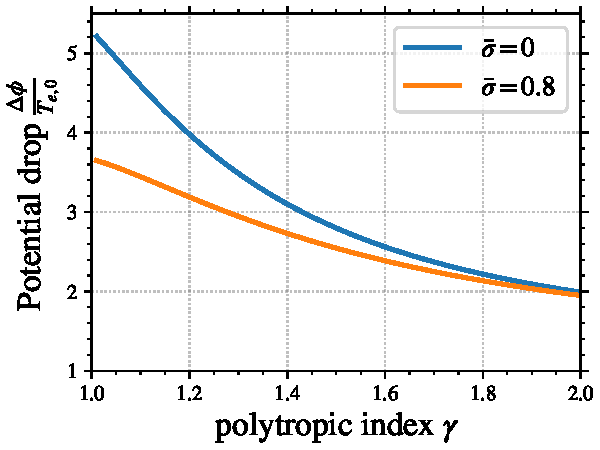
\includegraphics[width=\defaultwidth]{Sheath_drop_with_SEE.pdf}
  \caption{Potential drop $\dphi$ normilized by the bulk electron temperature $\Te_0$ as a function of the polytropic index $\gamma$ for a xenon plasma ($m_i = 131\,\atomicmass$). The emission rate $\rate$ is fixed for clarity.}
  \label{fig-dphi_see}
\end{figure}

The electron emission rate is actually a function of the electron energy at the wall.
Hence, using the same hypothesis that used in \cref{eq-ge}, we can compute the emission rate with \cref{eq-seemaxw}
\begin{equation} \label{eq-seemaxw_poly}
  \rate = \ratemaxw(\Tew) = \sigo + ( 1 - \sigo) \frac{ 2 \Tew  }{\crover}.
\end{equation}
Combined with \cref{eq-tew}, we obtain

\begin{equation} \label{eq-seemaxw_Tew}
  \rate = \sigo + ( 1 - \sigo) \frac{ 2 \lp \Teb - \frac{\gamma - 1}{\gamma} \dphi \rp }{\crover}.
\end{equation}
Here, we neglect the saluration of $\rate$ due to the \ac{SCL} regime.
\improvement{Calculated the SCL limit for polytropic !}

Noting $\chi = \frac{\gamma -1}{\gamma} \frac{ \dphi_0}{ \Te_0} $, we finely obtain the equation to be solved
\begin{equation} \label{eq-costseepoly}
  \left[ 1 + \chi  \right]^{\frac{1}{\gamma - 1}} \sqrt{1 - \chi} - \frac{ \crover \sqrt{4 \gamma m_e / m_i}}{ 2 \Teb (1 - \sigo) [1 -  (1 - \chi ) ] } = 0.
\end{equation}

\Cref{eq-costseepoly} depends explicitly on $\Teb$, hence $\chi$ is no longer independent of $\Teb$.
Moreover, the \ac{RHS} of \cref{eq-costseepoly} is more complex that before, leading to multiple solutions.
\Cref{fig-costfunction} shows the \ac{RHS} of \cref{eq-costseepoly} for several values of ({\bf a}) $\Teb$ and ({\bf b}) $\crover$, while keeping the polytropic index to $\gamma=1.35$.

The \ac{SCL} regime has been taken into account by saturating $\rate$ to $\ratecr=0.982$. 
It corresponds to the branch which crosses the abscissa axis close to $\frac{\dphi}{\Teb}=1$. 

\begin{figure}[hbtp]
  \centering
  \begin{tabular}{c c}
    \subfigure{cost_function_bis.pdf}{a}{20,20} &
    \subfigure{cost_function_2bis.pdf}{b}{20,20} \\
  \end{tabular}
  \caption{Value of the \ac{RHS} of \cref{eq-costseepoly}, labelled cost function, for several values of ({\bf a}) $\Teb$ and ({\bf b}) $\crover$.}
  \label{fig-costfunction}
\end{figure}

We can the that \cref{eq-costseepoly} can present two solutions, or no solutions, depending of the relative values of $crover$ and $\Teb$.
Hence, a particular care must be taken now when finding the sheath potential drop.

\Cref{fig-rso_crit_see} shows the evolution of the sheath potential drop with the electron temperature for different values of $\crover$.
It corresponds to \cref{fig-dphivsTe} with the use of a polytropic index.
We can see now that the electron temperature in the center $\Teb$ must be much higher before that the inversion of the plasma sheath potential, compared to \cref{fig-dphivsTe}.

\begin{figure}[hbtp]
  \centering
  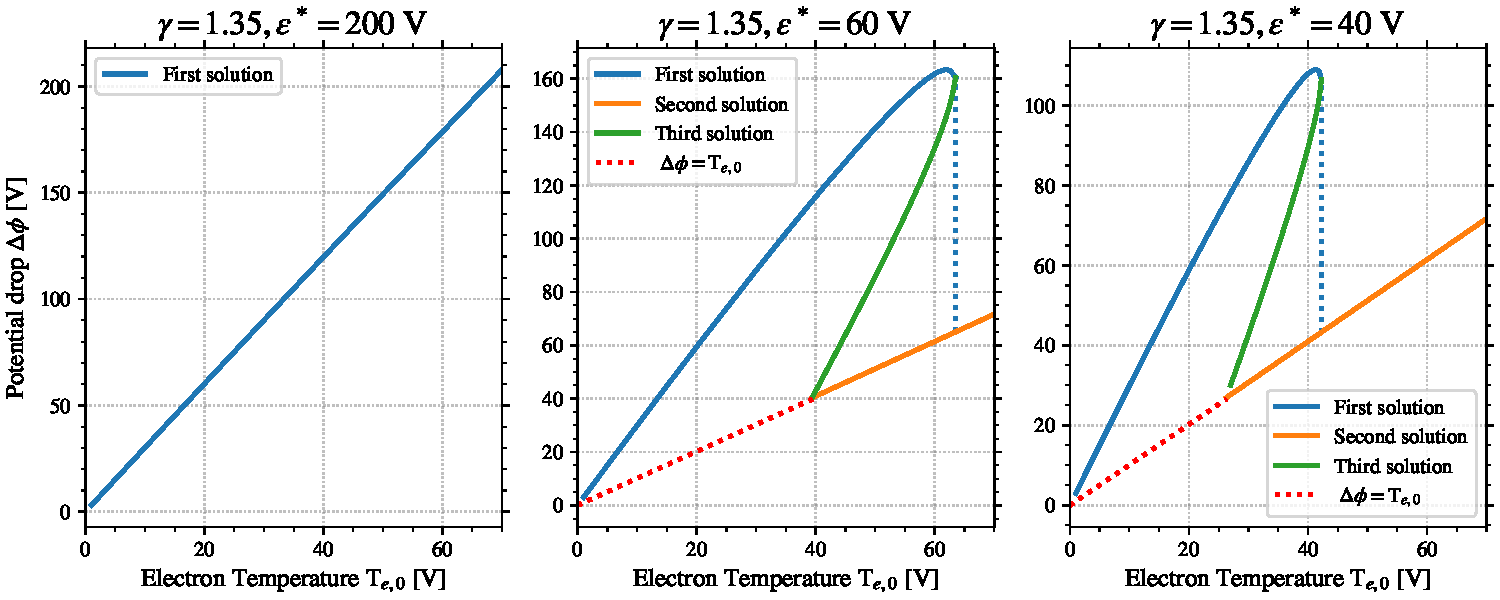
\includegraphics[width=\textwidth]{Potential_drop_poly_see.pdf}
  \caption{ Plasma potential drop to the wall as a function of the electron temperature for different values of the cross-over energy $\crover$ using \cref{eq-costseepoly}. It is the same results as  \cref{fig-dphivsTe} but with polytropic electron of index $\gamma=1.35$.}
  \label{fig-rso_crit_see}
\end{figure}

The electron temperature at inversion at $\crover=30\,\volt$ is around $\Teb=32\,\volt$, which is much closer to the mean electron temperature measured in regime {\bf II}.





\FloatBarrier

\section{Comparison with PIC simulations} \label{subsec-picandmodel}

\begin{figure}[hbtp]
  \centering
  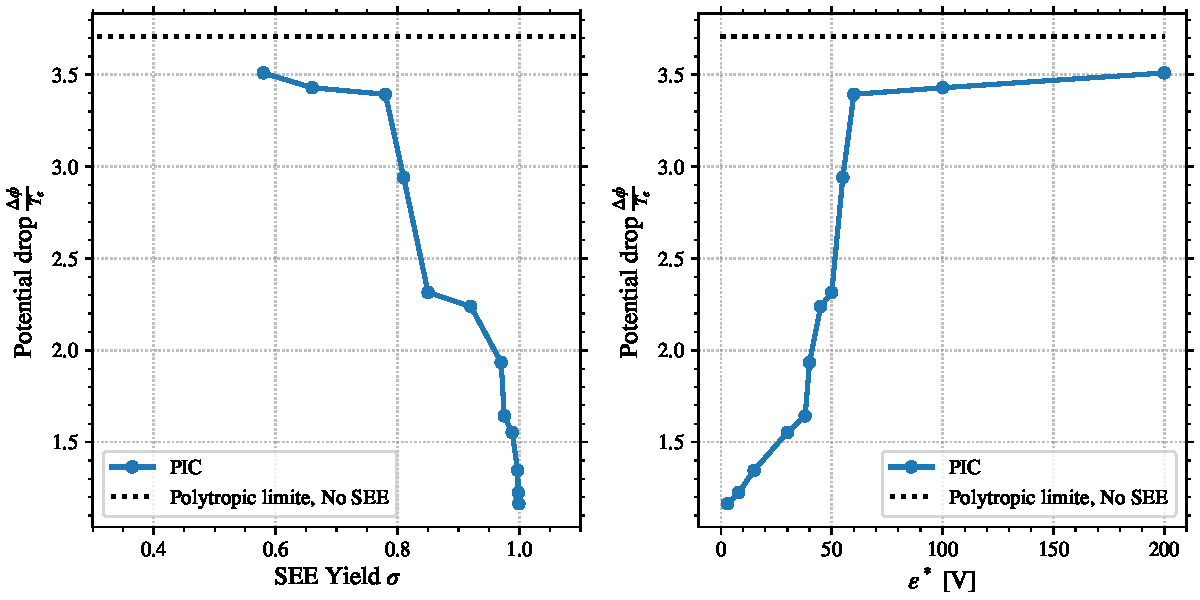
\includegraphics[width=\textwidth]{dphi_polytropic_noSEE}
  \caption{PIC simulation results (with SEE) compared to the polytropic limit without SEE.}
  \label{fig-polytropic_pic_noSEE}
\end{figure}

\begin{figure}[hbtp]
  \centering
  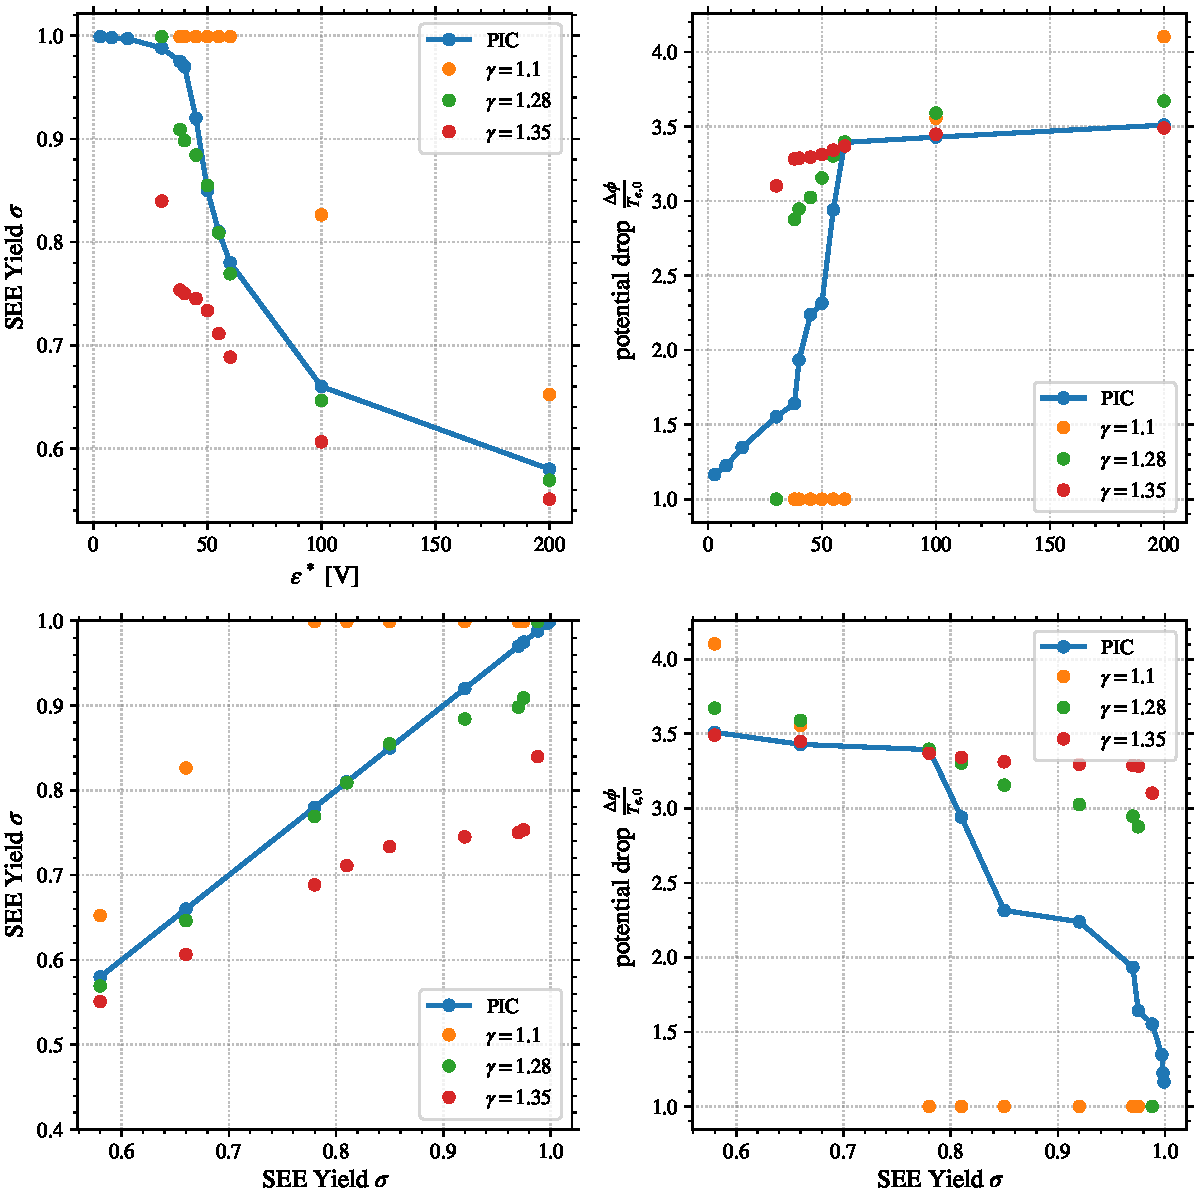
\includegraphics[width=\textwidth]{Summary_polytropic_SEE.pdf}
  \caption{Comparison of the PIC simulation results with the polytropic model with SEE.}
  \label{fig-polytropic_see_summary}
\end{figure}
